% ============================================================
%  يُترجَم بـ XeLaTeX  (في Overleaf: Menu → Compiler → XeLaTeX)
%  الخط: Amiri (متوفر في Overleaf، أو حمّله من github.com/aliftype/amiri)
% ============================================================
\documentclass[12pt,a4paper]{article}
\usepackage[a4paper,margin=1.7cm,top=2.3cm,bottom=2.9cm,headheight=15pt,footskip=1.5cm]{geometry}
\usepackage{amsmath,amssymb}
\usepackage{icomma}
\usepackage[english,bidi=default,layout=lists]{babel}
\babelprovide[import,main]{arabic}
\babelfont{rm}[Scale=1.08]{Amiri}
\babelfont{sf}[Scale=1.08]{Amiri}
\usepackage[most]{tcolorbox}
\usepackage{tikz}
\usetikzlibrary{arrows.meta,calc,shadings}
\usepackage{array}
\usepackage{colortbl}
\usepackage{fancyhdr}
\usepackage{titlesec}
\usepackage{enumitem}
\usepackage{collcell}
\usepackage{needspace}
\usepackage{etoolbox}
% أعمدة جداول تُكتب خلاياها بالعربية في الاتجاه الصحيح
\newcolumntype{C}{>{\collectcell\ar}c<{\endcollectcell}}
% تجنب عنوان يتيم في أسفل الصفحة
\pretocmd{\section}{\Needspace{15\baselineskip}}{}{}
\pretocmd{\subsection}{\Needspace{11\baselineskip}}{}{}

% ---------- الألوان ----------
\definecolor{cDef}{HTML}{1F4E9C}
\definecolor{cThm}{HTML}{B3261E}
\definecolor{cRem}{HTML}{2E7D32}
\definecolor{cEx}{HTML}{C76B00}
\definecolor{cMeth}{HTML}{6A1B9A}
\definecolor{cSol}{HTML}{00695C}
\definecolor{cSec}{HTML}{1F3A68}

% ---------- العناوين ----------
\titleformat{\section}{\Large\bfseries\color{cSec}}{\thesection.}{0.6em}{}[{\color{cSec!60}\titlerule[1pt]}]
\titleformat{\subsection}{\large\bfseries\color{cThm!85!black}}{\thesubsection.}{0.5em}{}
\titlespacing*{\section}{0pt}{14pt}{8pt}
\titlespacing*{\subsection}{0pt}{10pt}{5pt}
\setlength{\parindent}{0pt}
\setlength{\parskip}{4pt}
\setlist{itemsep=2pt,topsep=3pt}

% ---------- الصناديق (تُرسم في سياق LTR ويُكتب محتواها بالعربية) ----------
\newtcolorbox{arbox}[3][]{enhanced,
  colback=#2!5,colframe=#2!80!black,arc=2mm,boxrule=0.8pt,
  left=6pt,right=6pt,top=8pt,bottom=5pt,
  fonttitle=\bfseries,coltitle=white,
  title={\foreignlanguage{arabic}{#3}},
  attach boxed title to top right={xshift=-5mm,yshift=-3mm},
  boxed title style={colback=#2!80!black,arc=1.5mm,boxrule=0pt},
  before upper={\selectlanguage{arabic}},
  before skip=8pt,after skip=8pt,breakable,#1}
\newenvironment{BOX}[2]{\begin{otherlanguage}{english}\begin{arbox}{#1}{#2}}{\end{arbox}\end{otherlanguage}}
\newenvironment{tarif}[1][تعريف]{\begin{BOX}{cDef}{#1}}{\end{BOX}}
\newenvironment{khassia}[1][خاصية]{\begin{BOX}{cThm}{#1}}{\end{BOX}}
\newenvironment{molahada}[1][ملاحظة]{\begin{BOX}{cRem}{#1}}{\end{BOX}}
\newenvironment{mithal}[1][مثال]{\begin{BOX}{cEx}{#1}}{\end{BOX}}
\newenvironment{tariqa}[1][طريقة]{\begin{BOX}{cMeth}{#1}}{\end{BOX}}

% ---------- التمارين والحلول ----------
\newcounter{exo}
\newenvironment{tamrin}[1]{\stepcounter{exo}\begin{BOX}{cSec}{التمرين \theexo: #1}}{\end{BOX}}
\newenvironment{hal}{\Needspace{12\baselineskip}\begin{otherlanguage}{english}\begin{arbox}[breakable]{cSol}{حل التمرين \theexo}}{\end{arbox}\end{otherlanguage}}

% رسومات TikZ تُوضع في سياق LTR
\newenvironment{LTR}{\begin{otherlanguage}{english}}{\end{otherlanguage}}
\newcommand{\ar}[1]{\foreignlanguage{arabic}{#1}}

% ---------- رموز ----------
% نقاط الحذف داخل الرياضيات (\dots يسبب خللاً في الاتجاه مع babel)
\renewcommand{\dots}{\mathinner{\ldotp\ldotp\ldotp}}
\renewcommand{\ldots}{\mathinner{\ldotp\ldotp\ldotp}}
\renewcommand{\cdots}{\mathinner{\cdotp\cdotp\cdotp}}
\newcommand{\N}{\mathbb{N}}
\newcommand{\Z}{\mathbb{Z}}
\newcommand{\D}{\mathbb{D}}
\newcommand{\Q}{\mathbb{Q}}
\newcommand{\R}{\mathbb{R}}
\newcommand{\pgcd}{\operatorname{PGCD}}
\newcommand{\ppcm}{\operatorname{PPCM}}

% ---------- تمثيل مجال على مستقيم عددي ----------
% \NLseg{a}{b}{[}{]}  مجال محدود
\newcommand{\NLseg}[4]{\begin{LTR}\begin{tikzpicture}[baseline=-0.6ex]
 \draw[-{Stealth[length=2mm]},gray!70](0,0)--(3.4,0);
 \draw[line width=2pt,cThm!80!black](0.7,0)--(2.7,0);
 \node[cThm!80!black,font=\LARGE] at (0.7,0){$#3$};
 \node[cThm!80!black,font=\LARGE] at (2.7,0){$#4$};
 \node[below=3pt,font=\footnotesize] at (0.7,0){$#1$};
 \node[below=3pt,font=\footnotesize] at (2.7,0){$#2$};
\end{tikzpicture}\end{LTR}}
% \NLright{a}{[}  مجال نحو +∞
\newcommand{\NLright}[2]{\begin{LTR}\begin{tikzpicture}[baseline=-0.6ex]
 \draw[-{Stealth[length=2mm]},gray!70](0,0)--(3.4,0);
 \draw[line width=2pt,cThm!80!black](1.3,0)--(3.3,0);
 \node[cThm!80!black,font=\LARGE] at (1.3,0){$#2$};
 \node[below=3pt,font=\footnotesize] at (1.3,0){$#1$};
\end{tikzpicture}\end{LTR}}
% \NLleft{b}{]}  مجال نحو −∞
\newcommand{\NLleft}[2]{\begin{LTR}\begin{tikzpicture}[baseline=-0.6ex]
 \draw[-{Stealth[length=2mm]},gray!70](0,0)--(3.4,0);
 \draw[line width=2pt,cThm!80!black](0.05,0)--(2.1,0);
 \node[cThm!80!black,font=\LARGE] at (2.1,0){$#2$};
 \node[below=3pt,font=\footnotesize] at (2.1,0){$#1$};
\end{tikzpicture}\end{LTR}}

% ---------- أيقونات مواقع التواصل (مرسومة بـ TikZ، لا تحتاج أي حزمة) ----------
\definecolor{cFB}{HTML}{1877F2}
\definecolor{cTG}{HTML}{229ED9}
\definecolor{cIG1}{HTML}{FEDA75}
\definecolor{cIG2}{HTML}{D62976}
\definecolor{cIG3}{HTML}{4F5BD5}
\newcommand{\fbicon}{\begin{LTR}\begin{tikzpicture}[baseline=-0.75ex,x=1em,y=1em]
 \fill[cFB] (0,0) circle (0.55);
 \node[white,inner sep=0,font=\usefont{TU}{lmss}{bx}{n}\small] at (0.04,-0.02) {f};
\end{tikzpicture}\end{LTR}}
\newcommand{\igicon}{\begin{LTR}
\begin{tikzpicture}[baseline=-0.75ex,x=1em,y=1em]
 \shade[lower left=cIG1,lower right=cIG2,upper left=cIG2,upper right=cIG3,rounded corners=0.28em] (-0.55,-0.55) rectangle (0.55,0.55);
 \draw[white,line width=0.09em,rounded corners=0.18em] (-0.36,-0.36) rectangle (0.36,0.36);
 \draw[white,line width=0.09em] (0,0) circle (0.17);
 \fill[white] (0.22,0.22) circle (0.05);
\end{tikzpicture}\end{LTR}}
\newcommand{\tgicon}{\begin{LTR}
\begin{tikzpicture}[baseline=-0.75ex,x=1em,y=1em]
 \fill[cTG] (0,0) circle (0.55);
 \fill[white] (-0.33,0.0) -- (0.32,0.27) -- (0.2,-0.3) -- (0.0,-0.15) -- (-0.08,-0.28) -- (-0.08,-0.08) -- cycle;
 \fill[cTG!70!black] (-0.08,-0.08) -- (0.25,0.2) -- (0.0,-0.15) -- (-0.08,-0.28) -- cycle;
\end{tikzpicture}\end{LTR}}
% سطر مواقع التواصل أسفل كل صفحة
% (يُكتب السطر بترتيب بصري من اليسار إلى اليمين: الأيقونة يمين كل اسم)
\newcommand{\PageBox}{\begin{LTR}\tikz[baseline=(p.base)]\node[fill=black,text=white,inner sep=2.5pt,minimum width=1.6em,minimum height=1.3em,font=\usefont{TU}{lmss}{bx}{n}\small](p){\ifnum\value{page}<10 0\fi\arabic{page}};\end{LTR}}
\newcommand{\SocialRow}{\begin{otherlanguage}{english}%
 \ar{\textbf{الأستاذ سوايسية هشام للرياضيات}}\ \tgicon\hfill
 \textbf{prof\_hicham\_math}\ \igicon\hfill
 \ar{\textbf{الأستاذ سوايسية هشام للرياضيات}}\ \fbicon\hspace{2.2em}\PageBox\end{otherlanguage}}
% ---------- رأس وتذييل الصفحة ----------
\pagestyle{fancy}
\fancyhf{}
\renewcommand{\headrulewidth}{0.6pt}
\renewcommand{\footrulewidth}{0.4pt}
% \SetHeader{يمين الرأس}{يسار الرأس}{يمين التذييل}{يسار التذييل}
\newcommand{\SetHeader}[2]{%
 \fancyhead[C]{\parbox{\textwidth}{\ar{#1\hfill #2}}}%
 \fancyfoot[C]{\parbox{\textwidth}{\small\SocialRow}}}

\usepackage{tkz-tab}
\usepackage{multicol}
% جدول تغيرات / إشارة (يُرسم في سياق LTR)
\newenvironment{TAB}{\par\begin{center}\begin{LTR}\begin{tikzpicture}[scale=0.95,every node/.style={font=\small}]}{\end{tikzpicture}\end{LTR}\end{center}}
% معلم بشبكة: \begin{GR}{xmin}{xmax}{ymin}{ymax}{unit cm}
\newenvironment{GR}[5]{\par\begin{center}\begin{LTR}\begin{tikzpicture}[x=#5cm,y=#5cm,font=\footnotesize]
 \def\xmn{#1}\def\xmx{#2}\def\ymn{#3}\def\ymx{#4}
 \draw[gray!25,very thin] (#1,#3) grid (#2,#4);
 \draw[-{Stealth[length=2mm]}] (#1,0)--(#2+0.3,0) node[below left]{$x$};
 \draw[-{Stealth[length=2mm]}] (0,#3)--(0,#4+0.3) node[below left]{$y$};
 \node[below left] at (0,0){$O$};
 \draw[very thick,-{Stealth[length=1.6mm]}] (0,0)--(1,0) node[below,pos=.55]{$\vec i$};
 \draw[very thick,-{Stealth[length=1.6mm]}] (0,0)--(0,1) node[left,pos=.55]{$\vec j$};
 \begin{scope}\clip (#1,#3) rectangle (#2,#4);}
{\end{scope}\end{tikzpicture}\end{LTR}\end{center}}
\newcommand{\Ticks}[2]{\foreach \t in {#1} \node[below,font=\scriptsize] at (\t,0){$\t$}; \foreach \t in {#2} \node[left,font=\scriptsize] at (0,\t){$\t$};}
\newcommand{\bx}[1]{\ensuremath{\colorbox{cDef!12}{$\displaystyle #1$}}}
\newcommand{\hl}[1]{\ensuremath{\colorbox{cEx!20}{$\displaystyle #1$}}}
\newcommand{\Lim}[1]{\displaystyle\lim_{x\to #1}}
\newcommand{\Cf}{(C_f)}
\newenvironment{qst}{\begin{enumerate}[label=\protect\circled{\arabic*},leftmargin=*]}{\end{enumerate}}
\newcommand{\circled}[1]{\foreignlanguage{english}{\tikz[baseline=(c.base)]\node[circle,fill=cDef,text=white,inner sep=1.2pt,font=\scriptsize\bfseries](c){#1};}}
% عمودان: \TwoCol{عرض اليسار}{محتوى اليسار}{عرض اليمين}{محتوى اليمين}  (آمن مع TikZ)
\newcommand{\TwoCol}[4]{\par\begin{LTR}\noindent\begin{minipage}[t]{#1\textwidth}\selectlanguage{arabic}#2\end{minipage}\hfill\begin{minipage}[t]{#3\textwidth}\selectlanguage{arabic}#4\end{minipage}\end{LTR}\par}
\newcommand{\un}{(u_n)}\newcommand{\vn}{(v_n)}
% برهان بالتراجع: \Rec{الخاصية P(n)}{التحقق من P(0)}{البرهان على الوراثة}
\newcommand{\Rec}[3]{\textbf{برهان بالتراجع:} نسمي $P(n)$ الخاصية: «#1».
\begin{itemize}
\item \textbf{التحقق:} #2
\item \textbf{الوراثة:} نفرض أن $P(n)$ صحيحة ونبرهن صحة $P(n+1)$: #3
\item \textbf{الخلاصة:} حسب مبدأ الاستدلال بالتراجع، $P(n)$ صحيحة من أجل كل عدد طبيعي $n$.
\end{itemize}}
\newcommand{\src}[1]{{\footnotesize\textbf{#1}}\par}
\newcommand{\ok}{$\textcolor{cRem}{\checkmark}$}
\newcommand{\limn}{\displaystyle\lim_{n\to+\infty}}
% أسئلة فرعية (أ) (ب) (جـ) كل سؤال في سطر
\newenvironment{sq}{\begin{itemize}[leftmargin=2.4em,itemsep=3pt]}{\end{itemize}}
\newcommand{\qa}{\item[(أ)]}\newcommand{\qb}{\item[(ب)]}\newcommand{\qc}{\item[(جـ)]}\newcommand{\qd}{\item[(د)]}\newcommand{\qe}{\item[(هـ)]}
\newcommand{\pa}{\par\smallskip\textbf{(أ)} }\newcommand{\pb}{\par\smallskip\textbf{(ب)} }\newcommand{\pc}{\par\smallskip\textbf{(جـ)} }\newcommand{\pd}{\par\smallskip\textbf{(د)} }\newcommand{\pe}{\par\smallskip\textbf{(هـ)} }
\newcommand{\ccl}[1]{\par\textbf{الخلاصة:} #1}

\SetHeader{\small\bfseries\color{cSec}ملخص: عموميات على الدوال}{\small\color{cSec}السنة الأولى ثانوي -- جذع مشترك علوم وتكنولوجيا}
\begin{document}
\newcolumntype{M}[1]{>{\centering\arraybackslash}p{#1}}
\newcommand{\RL}[4]{\TwoCol{#3}{#4}{#1}{#2}}
\newcommand{\QQ}[1]{\par\smallskip\textbf{#1.} }
\newenvironment{tmr}{\stepcounter{exo}\begin{BOX}{cSec}{تمرين محلول \theexo}}{\end{BOX}}
\newcommand{\Df}{D_f}
\newcommand{\Tag}[2]{\foreignlanguage{english}{\tcbox[on line,colback=#1!15,colframe=#1,boxrule=0.6pt,arc=2pt,boxsep=0pt,left=3pt,right=3pt,top=1pt,bottom=1pt]{\ar{\textbf{#2}}}}}
\begin{LTR}
\begin{tcolorbox}[enhanced,colback=cSec,colframe=cSec,arc=3mm,halign=center,boxrule=0pt,top=12pt,bottom=12pt,before upper={\selectlanguage{arabic}}]
{\color{white}\fontsize{28}{34}\selectfont\bfseries عموميات على الدوال}\\[8pt]
{\color{white}\large ملخص شامل مع أمثلة وأشكال وتمارين محلولة خطوة بخطوة}\\[5pt]
{\color{white}\large السنة الأولى ثانوي -- جذع مشترك علوم وتكنولوجيا}
\end{tcolorbox}
\end{LTR}
\begin{BOX}{cDef}{محتوى الملخص}
\begin{center}
\begin{tabular}{p{0.44\textwidth}p{0.44\textwidth}}
5. اتجاه تغير دالة وجدول التغيرات & 1. مفهوم الدالة: الصورة والسابقة\\
6. القيم الحدية (القيم القصوى) & 2. مجموعة تعريف دالة\\
7. الحل البياني لمعادلات ومتراجحات & 3. التمثيل البياني والقراءة البيانية\\
8. خلاصة الطرائق & 4. الدالة الزوجية والدالة الفردية
\end{tabular}
\end{center}
\end{BOX}

% =====================================================================
\section{مفهوم الدالة: الصورة والسابقة}
\begin{tarif}
$D$ جزء من $\R$. \ \textbf{الدالة} $f$ المعرّفة على $D$ هي علاقة ترفق بكل عدد حقيقي $x$ من $D$ عدداً حقيقياً \textbf{وحيداً} نرمز له بـ $f(x)$. \ نكتب:
\[f:\ D\longrightarrow\R\qquad;\qquad x\longmapsto f(x).\]
\begin{itemize}
\item العدد $f(x)$ يسمى \textbf{صورة} $x$ بالدالة $f$.
\item إذا كان $f(a)=b$ فإن $a$ يسمى \textbf{سابقة} (أو سابقاً) للعدد $b$ بالدالة $f$.
\end{itemize}
\end{tarif}
\begin{molahada}
\begin{itemize}
\item لكل عدد $x$ من $D$ \textbf{صورة واحدة فقط}.
\item قد يكون لعدد $b$ سابقة واحدة ، أو عدة سوابق ، أو لا يكون له أي سابقة.
\item لإيجاد صورة $a$: نحسب $f(a)$. \ لإيجاد سوابق $b$: نحل المعادلة $f(x)=b$.
\end{itemize}
\end{molahada}
\begin{mithal}
$f(x)=x^2-3$ معرّفة على $\R$.
\begin{itemize}
\item صورة $2$: $f(2)=4-3=\bx{1}$ ، \ وصورة $-2$: $f(-2)=1$ أيضاً.
\item سوابق $6$: $x^2-3=6\iff x^2=9\iff x=3$ أو $x=-3$: للعدد $6$ \textbf{سابقتان} هما $3$ و $-3$.
\item سوابق $-5$: $x^2=-2$ مستحيلة ، إذن $-5$ \textbf{ليس له سابقة}.
\end{itemize}
\end{mithal}

% =====================================================================
\section{مجموعة تعريف دالة}
\begin{tarif}
\textbf{مجموعة تعريف} الدالة $f$ ، ونرمز لها بـ $\Df$ ، هي مجموعة الأعداد الحقيقية $x$ التي يكون من أجلها $f(x)$ قابلاً للحساب.
\end{tarif}
\begin{khassia}[قواعد التعيين]
\begin{itemize}
\item \textbf{كثير حدود} (مثل $3x^2-x+1$): \ معرّفة على $\R$.
\item \textbf{كسر} $\dfrac{A(x)}{B(x)}$: \ نشترط $B(x)\ne0$ (المقام غير معدوم).
\item \textbf{جذر تربيعي} $\sqrt{A(x)}$: \ نشترط $A(x)\ge0$.
\item \textbf{جذر في المقام} $\dfrac{1}{\sqrt{A(x)}}$: \ نشترط $A(x)>0$.
\end{itemize}
\end{khassia}
\begin{mithal}
\begin{itemize}
\item $f(x)=\dfrac{2x+1}{x-3}$: \ $x-3\ne0\iff x\ne3$ ، \ \bx{D_f=\R-\{3\}=\,]-\infty;3[\,\cup\,]3;+\infty[}.
\item $g(x)=\dfrac{5}{x^2-1}$: \ $x^2-1=0\iff x=1$ أو $x=-1$ ، \ \bx{D_g=\R-\{-1;1\}}.
\item $h(x)=\sqrt{4-2x}$: \ $4-2x\ge0\iff x\le2$ ، \ \bx{D_h=\,]-\infty;2]}.
\item $k(x)=\dfrac{\sqrt{x+1}}{x-2}$: \ $x+1\ge0$ و $x\ne2$ ، \ \bx{D_k=[-1;2[\,\cup\,]2;+\infty[}.
\end{itemize}
\end{mithal}

% =====================================================================
\section{التمثيل البياني والقراءة البيانية}
\begin{tarif}
المستوي منسوب إلى معلم $(O;\vec i,\vec j)$. \ \textbf{التمثيل البياني} (أو المنحنى الممثل) للدالة $f$ هو مجموعة النقط $M(x;y)$ حيث $x\in\Df$ و $y=f(x)$. \ نرمز له بـ $(C_f)$ ، ونقول إن $y=f(x)$ \textbf{معادلة} له.
\[M(x;y)\in(C_f)\iff x\in\Df\ \text{\ar{و}}\ y=f(x).\]
\end{tarif}
\begin{tariqa}[قراءة صورة عدد بيانياً (الأسهم: محور الفواصل $\to$ المنحنى $\to$ محور التراتيب)]
\RL{0.5}{%
لقراءة صورة العدد $a$:
\begin{enumerate}
\item نعلّم $a$ على \textbf{محور الفواصل}.
\item نصعد (أو ننزل) \textbf{شاقولياً} حتى نلتقي بالمنحنى $(C_f)$.
\item نتجه \textbf{أفقياً} نحو \textbf{محور التراتيب}: العدد المقروء هو $f(a)$.
\end{enumerate}
\Tag{cDef}{بالأزرق}: ننطلق من $-1$ ، نصعد إلى $(C_f)$ ثم نتجه أفقياً فنقرأ \bx{f(-1)=2}.\par
\Tag{cEx}{بالبرتقالي}: ننطلق من $1$ ، ننزل إلى $(C_f)$ ثم نتجه أفقياً فنقرأ \bx{f(1)=-2}.\par
لكل عدد $a$ من $D_f$ \textbf{صورة واحدة}: المستقيم الشاقولي يقطع المنحنى في نقطة واحدة.}{0.47}{%
\begin{LTR}\centering
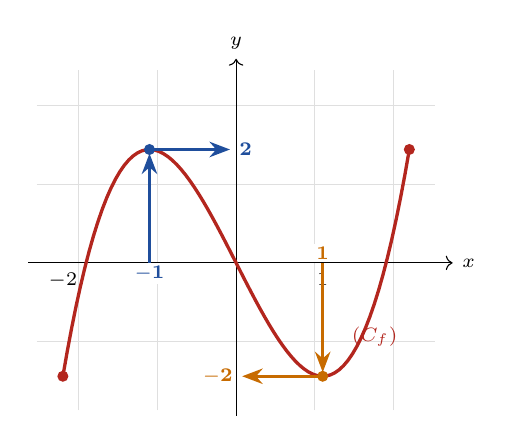
\begin{tikzpicture}[x=1.1cm,y=0.72cm,font=\scriptsize,
 ar/.style={very thick,-{Stealth[length=2.6mm]}}]
\draw[gray!25] (-2.3,-2.6) grid (2.3,3.4);
\draw[->] (-2.4,0)--(2.5,0) node[right]{$x$}; \draw[->] (0,-2.7)--(0,3.6) node[above]{$y$};
\foreach \x in {-2,1} \node[below] at (\x,0){$\x$};
\draw[cThm,very thick,domain=-2:2,samples=80] plot (\x,{\x*\x*\x-3*\x});
\fill[cThm] (-2,-2) circle (2pt) (2,2) circle (2pt);
\node[cThm] at (1.6,-1.3){$(C_f)$};
\draw[cDef,ar] (-1,0)--(-1,1.93);
\draw[cDef,ar] (-1,2)--(-0.07,2);
\fill[cDef] (-1,2) circle (2pt);
\node[cDef,below,fill=white,inner sep=1pt] at (-1,0){$\mathbf{-1}$};
\node[cDef,right,fill=white,inner sep=1pt] at (0,2){$\mathbf{2}$};
\draw[cEx,ar] (1,0)--(1,-1.93);
\draw[cEx,ar] (1,-2)--(0.07,-2);
\fill[cEx] (1,-2) circle (2pt);
\node[cEx,left,fill=white,inner sep=1pt] at (0,-2){$\mathbf{-2}$};
\node[cEx,above,fill=white,inner sep=1pt] at (1,0){$\mathbf{1}$};
\end{tikzpicture}
\end{LTR}}
\end{tariqa}

\begin{tariqa}[قراءة سوابق عدد بيانياً (الأسهم: محور التراتيب $\to$ المنحنى $\to$ محور الفواصل)]
\RL{0.5}{%
لقراءة سوابق العدد $b$:
\begin{enumerate}
\item نعلّم $b$ على \textbf{محور التراتيب} ونرسم \textbf{المستقيم الأفقي} $y=b$.
\item من \textbf{كل} نقطة تقاطع لهذا المستقيم مع $(C_f)$ ننزل (أو نصعد) \textbf{شاقولياً} نحو \textbf{محور الفواصل}.
\item الفواصل المقروءة هي سوابق $b$.
\end{enumerate}
\Tag{cRem}{بالأخضر}: المستقيم $y=2$ يقطع $(C_f)$ في نقطتين ، إذن للعدد $2$ \textbf{سابقتان}: \bx{-1} و \bx{2}.\par
\Tag{cMeth}{بالبنفسجي}: المستقيم $y=3$ لا يقطع $(C_f)$ ، إذن العدد $3$ \textbf{ليس له سابقة}.\par
عدد السوابق $=$ عدد نقط تقاطع $(C_f)$ مع المستقيم $y=b$ (قد يكون $0$ أو $1$ أو أكثر).}{0.47}{%
\begin{LTR}\centering
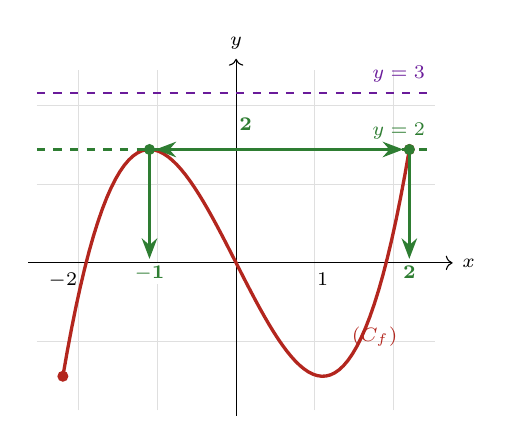
\begin{tikzpicture}[x=1.1cm,y=0.72cm,font=\scriptsize,
 ar/.style={very thick,-{Stealth[length=2.6mm]}}]
\draw[gray!25] (-2.3,-2.6) grid (2.3,3.4);
\draw[->] (-2.4,0)--(2.5,0) node[right]{$x$}; \draw[->] (0,-2.7)--(0,3.6) node[above]{$y$};
\foreach \x in {-2,1} \node[below] at (\x,0){$\x$};
\draw[cThm,very thick,domain=-2:2,samples=80] plot (\x,{\x*\x*\x-3*\x});
\fill[cThm] (-2,-2) circle (2pt) (2,2) circle (2pt);
\node[cThm] at (1.6,-1.3){$(C_f)$};
\draw[cRem,dashed,thick] (-2.3,2)--(2.3,2) node[above left]{$y=2$};
\draw[cRem,ar] (0,2)--(-0.93,2); \draw[cRem,ar] (0,2)--(1.93,2);
\draw[cRem,ar] (-1,2)--(-1,0.07); \draw[cRem,ar] (2,2)--(2,0.07);
\fill[cRem] (-1,2) circle (2pt) (2,2) circle (2pt);
\node[cRem,right,fill=white,inner sep=1pt] at (0,2.45){$\mathbf{2}$};
\node[cRem,below,fill=white,inner sep=1pt] at (-1,0){$\mathbf{-1}$};
\node[cRem,below,fill=white,inner sep=1pt] at (2,0){$\mathbf{2}$};
\draw[cMeth,dashed,thick] (-2.3,3)--(2.3,3) node[above left]{$y=3$};
\end{tikzpicture}
\end{LTR}}
\end{tariqa}

\begin{mithal}[قراءة بيانية]
\RL{0.5}{%
$(C_f)$ هو منحنى دالة $f$ معرّفة على $[-2;2]$.
\begin{itemize}
\item \textbf{الصورة:} نقرأ الترتيب: $f(-1)=2$ ، $f(0)=0$ ، $f(1)=-2$.
\item \textbf{السوابق:} سوابق العدد $2$ هي فواصل نقط تقاطع $(C_f)$ مع المستقيم $y=2$: $-1$ و $2$.
\item \textbf{حلول} $f(x)=0$: فواصل نقط تقاطع $(C_f)$ مع محور الفواصل: $-\sqrt3$ ، $0$ ، $\sqrt3$ (أي تقريباً $\pm1{,}7$).
\item \textbf{مجموعة الصور:} $[-2;2]$.
\end{itemize}}{0.47}{%
\begin{LTR}\centering
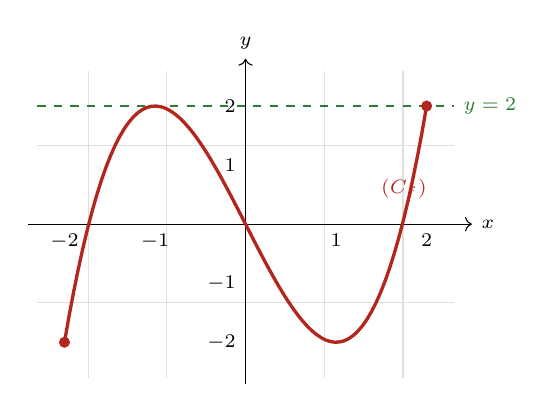
\begin{tikzpicture}[x=1.15cm,y=0.75cm,font=\scriptsize]
\draw[gray!25] (-2.3,-2.6) grid (2.3,2.6);
\draw[->] (-2.4,0)--(2.5,0) node[right]{$x$}; \draw[->] (0,-2.7)--(0,2.8) node[above]{$y$};
\foreach \x in {-2,-1,1,2} \node[below] at (\x,0){$\x$};
\foreach \y in {-2,-1,1,2} \node[left] at (0,\y){$\y$};
\draw[cRem,dashed] (-2.3,2)--(2.3,2) node[right]{$y=2$};
\draw[cThm,very thick,domain=-2:2,samples=80] plot (\x,{\x*\x*\x-3*\x});
\fill[cThm] (-2,-2) circle (2pt) (2,2) circle (2pt);
\node[cThm] at (1.75,0.6){$(C_f)$};
\end{tikzpicture}
\end{LTR}}
\end{mithal}
\begin{molahada}
النقطة $A(a;b)$ تنتمي إلى $(C_f)$ إذا وفقط إذا كان $a\in\Df$ و $f(a)=b$. \ مثال: $f(x)=x^2-3$ ، $A(2;1)\in(C_f)$ لأن $f(2)=1$ ، و $B(1;0)\notin(C_f)$ لأن $f(1)=-2\ne0$.
\end{molahada}

% =====================================================================
\section{الدالة الزوجية والدالة الفردية}
\begin{tarif}
$f$ دالة مجموعة تعريفها $\Df$ \textbf{متناظرة بالنسبة إلى الصفر} (أي: من أجل كل $x\in\Df$ يكون $-x\in\Df$).
\begin{itemize}
\item $f$ \textbf{زوجية} إذا كان من أجل كل $x\in\Df$: \ \bx{f(-x)=f(x)}.
\item $f$ \textbf{فردية} إذا كان من أجل كل $x\in\Df$: \ \bx{f(-x)=-f(x)}.
\end{itemize}
\end{tarif}
\begin{khassia}[التفسير البياني]
\RL{0.5}{%
\begin{itemize}
\item $f$ زوجية $\iff$ $(C_f)$ \textbf{متناظر بالنسبة إلى محور التراتيب}.
\item $f$ فردية $\iff$ $(C_f)$ \textbf{متناظر بالنسبة إلى المبدأ $O$}.
\end{itemize}}{0.47}{%
\begin{LTR}\centering
\begin{tikzpicture}[scale=0.5,font=\scriptsize]
\draw[->] (-2.3,0)--(2.3,0); \draw[->] (0,-0.5)--(0,3.4);
\draw[cThm,thick,domain=-1.75:1.75] plot (\x,{\x*\x-0.2});
\node at (0,-1){زوجية};
\begin{scope}[xshift=5.5cm,yshift=1.4cm]
\draw[->] (-2.3,0)--(2.3,0); \draw[->] (0,-2)--(0,2);
\draw[cDef,thick,domain=-1.6:1.6,samples=50] plot (\x,{0.5*(\x*\x*\x-2*\x)});
\fill (0,0) circle (2pt) node[below left]{$O$};
\node at (0,-2.4){فردية};
\end{scope}
\end{tikzpicture}
\end{LTR}}
\end{khassia}
\begin{mithal}
\begin{itemize}
\item $f(x)=x^2+1$ ، $\Df=\R$ متناظرة: $f(-x)=(-x)^2+1=x^2+1=f(x)$: \ $f$ \textbf{زوجية}.
\item $g(x)=x^3-x$ ، $D_g=\R$: $g(-x)=-x^3+x=-(x^3-x)=-g(x)$: \ $g$ \textbf{فردية}.
\item $h(x)=x^2+x$: $h(-1)=0$ و $h(1)=2$ ، فـ $h(-1)\ne h(1)$ و $h(-1)\ne-h(1)$: \ $h$ \textbf{لا زوجية ولا فردية}.
\item $k(x)=\dfrac{1}{x-1}$: $D_k=\R-\{1\}$ ليست متناظرة ($-1\in D_k$ لكن $1\notin D_k$): \ $k$ \textbf{لا زوجية ولا فردية}.
\end{itemize}
\end{mithal}

% =====================================================================
\section{اتجاه تغير دالة وجدول التغيرات}
\begin{tarif}
$f$ دالة و $I$ مجال محتوى في $\Df$.
\begin{itemize}
\item $f$ \textbf{متزايدة تماماً} على $I$ إذا كان من أجل كل $a$ و $b$ من $I$: \ $a<b\Rightarrow f(a)<f(b)$ \ (الدالة تحافظ على الترتيب).
\item $f$ \textbf{متناقصة تماماً} على $I$ إذا كان من أجل كل $a$ و $b$ من $I$: \ $a<b\Rightarrow f(a)>f(b)$ \ (الدالة تعكس الترتيب).
\item $f$ \textbf{ثابتة} على $I$ إذا كان من أجل كل $a$ و $b$ من $I$: $f(a)=f(b)$.
\end{itemize}
\end{tarif}
\begin{tariqa}[طريقتان لدراسة اتجاه التغير]
\begin{enumerate}
\item \textbf{المقارنة المباشرة:} ننطلق من $a<b$ ونصل بعمليات متتالية على المتباينة إلى مقارنة $f(a)$ و $f(b)$.
\item \textbf{نسبة التغير:} من أجل $a\ne b$ في $I$ ندرس إشارة $\dfrac{f(b)-f(a)}{b-a}$: \ موجبة تماماً معناه $f$ متزايدة تماماً على $I$ ، وسالبة تماماً معناه $f$ متناقصة تماماً على $I$.
\end{enumerate}
\end{tariqa}
\begin{mithal}
\begin{itemize}
\item $f(x)=-3x+2$ على $\R$: إذا كان $a<b$ فإن $-3a>-3b$ ، ومنه $-3a+2>-3b+2$ ، أي $f(a)>f(b)$: \ $f$ \textbf{متناقصة تماماً على $\R$}.
\item $g(x)=x^2$ على $[0;+\infty[$: إذا كان $0\le a<b$ فإن $a^2<b^2$ (بالضرب في أعداد موجبة) ، أي $g(a)<g(b)$: \ \textbf{متزايدة تماماً}.
\item $h(x)=\dfrac1x$ على $]0;+\infty[$: \ $\dfrac{h(b)-h(a)}{b-a}=\dfrac{\frac1b-\frac1a}{b-a}=\dfrac{\frac{a-b}{ab}}{b-a}=\dfrac{-1}{ab}<0$ (لأن $ab>0$): \ $h$ \textbf{متناقصة تماماً}.
\end{itemize}
\end{mithal}
\begin{khassia}[جدول التغيرات]
نلخص اتجاه التغير في جدول: السهم الصاعد يعني متزايدة ، والنازل يعني متناقصة ، ونكتب في أطراف الأسهم الصور.\par
\textbf{مثال:} الدالة $f$ الممثلة في الفقرة 3 (على $[-2;2]$):
\begin{TAB}
\tkzTabInit[lgt=1.3,espcl=2]{$x$/0.7,$f(x)$/1.5}{$-2$,$-1$,$1$,$2$}
\tkzTabVar{-/$-2$,+/$2$,-/$-2$,+/$2$}
\end{TAB}
$f$ متزايدة تماماً على $[-2;-1]$ وعلى $[1;2]$ ، ومتناقصة تماماً على $[-1;1]$.
\end{khassia}
\begin{molahada}
\begin{itemize}
\item إذا كانت $f$ زوجية (أو فردية) يكفي دراستها على $\Df\cap[0;+\infty[$ ثم نستنتج بالتناظر: الزوجية \textbf{تعكس} اتجاه التغير ، والفردية \textbf{تحافظ} عليه.
\item لا نقول $f$ متناقصة على $]-\infty;0[\cup]0;+\infty[$ عندما تتناقص على كل مجال منهما (مثل $\dfrac1x$).
\end{itemize}
\end{molahada}

% =====================================================================
\section{القيم الحدية (القيم القصوى)}
\begin{tarif}
$f$ دالة معرّفة على مجال $I$ ، و $a\in I$.
\begin{itemize}
\item $f(a)$ \textbf{قيمة حدية عظمى} لـ $f$ على $I$ إذا كان من أجل كل $x\in I$: \ $f(x)\le f(a)$.
\item $f(a)$ \textbf{قيمة حدية صغرى} لـ $f$ على $I$ إذا كان من أجل كل $x\in I$: \ $f(x)\ge f(a)$.
\end{itemize}
\end{tarif}
\begin{tariqa}[إثبات أن $m$ قيمة حدية صغرى]
نبيّن أن $f(x)-m\ge0$ لكل $x\in I$ (غالباً بكتابة مربع) ، ونجد عدداً $a$ حيث $f(a)=m$.
\end{tariqa}
\begin{mithal}
\begin{itemize}
\item $f(x)=x^2-4x+5=(x-2)^2+1$: \ $(x-2)^2\ge0$ ، إذن $f(x)\ge1$ ، و $f(2)=1$: \ \bx{1} \textbf{قيمة حدية صغرى} لـ $f$ على $\R$ ، تبلغها عند $x=2$.
\item $g(x)=-x^2+2x+3=4-(x-1)^2\le4$ ، و $g(1)=4$: \ \bx{4} \textbf{قيمة حدية عظمى} لـ $g$ على $\R$ ، تبلغها عند $x=1$.
\end{itemize}
\end{mithal}
\begin{molahada}
من جدول التغيرات نقرأ القيم الحدية: الدالة الممثلة في الفقرة 3 قيمتها الحدية العظمى $2$ (عند $-1$ و $2$) ، والصغرى $-2$ (عند $-2$ و $1$).
\end{molahada}

% =====================================================================
\section{الحل البياني لمعادلات ومتراجحات}
\begin{khassia}
\begin{itemize}
\item حلول المعادلة $f(x)=k$ هي فواصل نقط تقاطع $(C_f)$ مع المستقيم الأفقي $y=k$.
\item حلول المعادلة $f(x)=g(x)$ هي فواصل نقط تقاطع $(C_f)$ و $(C_g)$.
\item حلول المتراجحة $f(x)>g(x)$ هي فواصل نقط $(C_f)$ الواقعة \textbf{فوق} $(C_g)$ (وتحته للمتراجحة $f(x)<g(x)$).
\item حلول $f(x)>0$ هي فواصل نقط $(C_f)$ الواقعة فوق محور الفواصل.
\end{itemize}
\end{khassia}
\begin{mithal}
\RL{0.52}{%
$f(x)=x^2$ و $g(x)=x+2$.\par
\textbf{بيانياً:} $(C_f)$ و $(C_g)$ يتقاطعان في $A(-1;1)$ و $B(2;4)$:\par
\begin{itemize}
\item حلول $f(x)=g(x)$: \ $S=\{-1;2\}$.
\item $(C_f)$ تحت $(C_g)$ بين $-1$ و $2$: حلول $f(x)<g(x)$ هي $S=\,]-1;2[$.
\end{itemize}
\textbf{جبرياً (تحقق):} $x^2-x-2=(x+1)(x-2)$ ، وهو سالب تماماً بين الجذرين $-1$ و $2$ \ok.}{0.45}{%
\begin{LTR}\centering
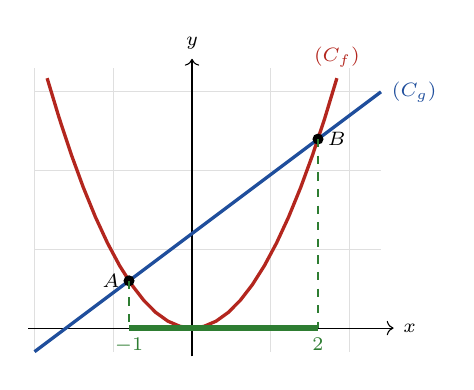
\begin{tikzpicture}[x=0.8cm,y=0.6cm,font=\scriptsize]
\draw[gray!25] (-2.5,-0.5) grid (3,5.5);
\draw[->] (-2.6,0)--(3.2,0) node[right]{$x$}; \draw[->] (0,-0.6)--(0,5.7) node[above]{$y$};
\draw[cThm,very thick,domain=-2.3:2.3] plot (\x,{\x*\x}) node[above]{$(C_f)$};
\draw[cDef,very thick] (-2.5,-0.5)--(3,5) node[right]{$(C_g)$};
\fill (-1,1) circle (2pt) node[left]{$A$}; \fill (2,4) circle (2pt) node[right]{$B$};
\draw[cRem,dashed] (-1,1)--(-1,0) node[below]{$-1$} (2,4)--(2,0) node[below]{$2$};
\draw[cRem,line width=2pt] (-1,0)--(2,0);
\end{tikzpicture}
\end{LTR}}
\end{mithal}

% =====================================================================
\section{تمرين محلول وخلاصة الطرائق}
\begin{tmr}
$f$ الدالة المعرّفة على $\R$ بـ: $f(x)=x^2-2x-3$.
\begin{enumerate}
\item احسب صورة $0$ و $-1$ ، ثم عيّن سوابق $-3$.
\item بيّن أنه من أجل كل $x$: $f(x)=(x-1)^2-4$ ، ثم استنتج القيمة الحدية الصغرى لـ $f$.
\item ادرس اتجاه تغير $f$ على $]-\infty;1]$ وعلى $[1;+\infty[$ ، ثم شكّل جدول تغيراتها.
\item هل $f$ زوجية؟
\end{enumerate}
\end{tmr}
\begin{hal}
\textbf{1.} $f(0)=\bx{-3}$ ، $f(-1)=1+2-3=\bx{0}$. \quad $f(x)=-3\iff x^2-2x=0\iff x(x-2)=0$: سوابق $-3$ هي \bx{0} و \bx{2}.
\QQ{2} $(x-1)^2-4=x^2-2x+1-4=x^2-2x-3=f(x)$ \ok. \ $(x-1)^2\ge0$ ، إذن $f(x)\ge-4$ و $f(1)=-4$: القيمة الحدية الصغرى \bx{-4} عند $x=1$.
\QQ{3} ليكن $a<b$:
\begin{itemize}
\item على $[1;+\infty[$: $1\le a<b\Rightarrow0\le a-1<b-1\Rightarrow(a-1)^2<(b-1)^2\Rightarrow f(a)<f(b)$: \ \textbf{متزايدة تماماً}.
\item على $]-\infty;1]$: $a<b\le1\Rightarrow a-1<b-1\le0\Rightarrow(a-1)^2>(b-1)^2\Rightarrow f(a)>f(b)$: \ \textbf{متناقصة تماماً}.
\end{itemize}
\begin{TAB}
\tkzTabInit[lgt=1.3,espcl=2.4]{$x$/0.7,$f(x)$/1.4}{$-\infty$,$1$,$+\infty$}
\tkzTabVar{+/,-/$-4$,+/}
\end{TAB}
\QQ{4} $f(-1)=0$ و $f(1)=-4$: $f(-1)\ne f(1)$ ، إذن $f$ \textbf{ليست زوجية} (منحناها متناظر بالنسبة إلى المستقيم $x=1$ وليس محور التراتيب).
\end{hal}
\begin{BOX}{cMeth}{ماذا أفعل عندما يُطلب مني $\ldots$؟}
\renewcommand{\arraystretch}{1.5}
\centering
\begin{tabular}{|p{0.56\textwidth}|p{0.32\textwidth}|}\hline
\cellcolor{cMeth!15}\textbf{الطريقة} & \cellcolor{cMeth!15}\textbf{المطلوب}\\\hline
نحسب $f(a)$ ، أو نقرأ ترتيب نقطة $(C_f)$ ذات الفاصلة $a$. & صورة العدد $a$\\\hline
نحل $f(x)=b$ ، أو نقرأ فواصل نقط تقاطع $(C_f)$ مع $y=b$. & سوابق العدد $b$\\\hline
نستبعد ما يعدم المقام ، ونشترط ما تحت الجذر موجباً. & مجموعة التعريف\\\hline
نتحقق من $a\in\Df$ و $f(a)=b$. & هل $A(a;b)\in(C_f)$؟\\\hline
نتحقق من تناظر $\Df$ ، ثم نحسب $f(-x)$ ونقارنه بـ $f(x)$ و $-f(x)$. & زوجية أو فردية\\\hline
ننطلق من $a<b$ ، أو ندرس إشارة $\dfrac{f(b)-f(a)}{b-a}$. & اتجاه التغير\\\hline
نكتب $f(x)=m+(\ldots)^2$ أو نقرأ جدول التغيرات. & القيمة الحدية\\\hline
فواصل نقط التقاطع ، أو مواضع المنحنى (فوق / تحت). & حل معادلة / متراجحة بيانياً\\\hline
\end{tabular}
\end{BOX}

\end{document}
